% !TeX program = xelatex
%!TEX TS-program = xelatex

% Официальный шаблон презентации НИУ ВШЭ в beamer (LaTeX)
% Версия 2.0
% Язык — русский

\documentclass[aspectratio=169,xcolor=dvipsnames]{beamer}

\newbool{russian}
\booltrue{russian}
\usepackage{HSE-theme/beamerthemeHSE}

%%% Работа с русским языком и шрифтами
\usepackage{multirow}
\usepackage{listings} 
\usepackage[english,russian,shorthands=off]{babel}
\usepackage[no-math]{fontspec}
\usepackage{makecell}
	\IfFontExistsTF{HSE Sans}
		{\newcommand{\presentationfont}{HSE Sans}}
		{\IfFontExistsTF{Arial}
          {\newcommand{\presentationfont}{Arial}}
          {\newcommand{\presentationfont}{Arimo}}}
	\setsansfont{\presentationfont}
	\IfFontExistsTF{Courier New}{\setmonofont{Courier New}}{\setmonofont{Liberation Mono}}

\usepackage[most]{tcolorbox}

\usepackage{mathspec}
	\setmathsfont(Digits,Latin,Greek)[Numbers={Lining,Proportional}]{\presentationfont}
	\setmathrm[Numbers={Lining,Proportional}]{\presentationfont}
\uselanguage{russian}
\languagepath{russian}
\deftranslation[to=russian]{Theorem}{Теорема}
\deftranslation[to=russian]{Definition}{Определение}
\deftranslation[to=russian]{Definitions}{Определения}
\deftranslation[to=russian]{Corollary}{Следствие}
\deftranslation[to=russian]{Fact}{Факт}
\deftranslation[to=russian]{Example}{Пример}
\deftranslation[to=russian]{Examples}{Примеры}

\usepackage{booktabs}
\usepackage{array}
\graphicspath{{images/}}


\newcommand{\term}[1]{{\large\textcolor{HSEblue}{#1}}}
\newcommand{\cmd}[1]{\textcolor{HSEblue}{\texttt{#1}}}
\lstset{ 
    basicstyle=\color{HSEblue}\ttfamily\small,
    numbers=left,
    numberstyle=\color{HSEblue}\ttfamily\scriptsize,
    frame=single,
    columns=fullflexible,
    keepspaces=true,
    showstringspaces=false,
    breaklines=true,
    rulecolor=\color{HSEblue},
}


%% Информация об авторе и выступлении

\title[Мобильные колесные роботы]{Одновременная локализация и картирование (SLAM)}
\subtitle{Проектный семинар <<Мобильные колесные роботы>>}
\author[Команда курса]{Дергачев Степан  Алексеевич, \texttt{\href{mailto:sadergachev@hse.ru}{sadergachev@hse.ru}} \\ Муравьев Кирилл Федорович, \texttt{\href{mailto:kmuravev@hse.ru}{kmuravev@hse.ru}}}
\institute{Факультет компьютерных наук НИУ ВШЭ}
\date{}



% Отключаем активные кавычки babel для совместимости с mathspec.
\AtBeginDocument{\shorthandoff{"}}
\makeatletter
\patchcmd{\beamer@@tmpl@footline}{\end{beamercolorbox} }{\end{beamercolorbox}}{}{}
\makeatother
\usepackage{tikz}
\usetikzlibrary{arrows.meta,positioning}
\newcommand{\source}[1]{\par\vfill{\fontsize{6}{7}\selectfont\color{gray}#1\par}}
%\newcommand{\mappingcredit}{\source{По материалам О. Шипитько. «Моделирование колесных роботов», МФТИ, 2020.}}
\newcommand{\fig}[2][4cm]{\includegraphics[width=\linewidth,height=#1,keepaspectratio]{slam/#2}}
% trim: слева, снизу, справа, сверху; единицы соответствуют пикселям исходника.
\newcommand{\screenfig}[3][4cm]{\includegraphics[width=\linewidth,height=#1,keepaspectratio,trim=#3,clip]{slam/#2}}
\begin{document}
% Слайд PPTX 1: титульный слайд адаптирован под курс.
\frame[plain]{\titlepage}

% Слайд PPTX 4
\begin{frame}
\frametitle{Задача картирования}
\begin{itemize}
\item \textcolor{HSEblue}{Картирование (mapping)} — процесс моделирования окружающей среды.
\item По данным с датчиков (измерениям) и состояниям робота требуется построить карту $m$.
\item Карта должна обеспечивать возможность навигации робота в среде:
	\begin{itemize}
		\item Локализация робота по карте;
		\item Планирование проходимых для робота маршрутов между точками среды.
	\end{itemize}
\end{itemize}
\end{frame}

% Слайд PPTX 5
\begin{frame}
\frametitle{Какие бывают карты?}
\small \begin{columns}[c]\column{.48\textwidth}\begin{block}{Метрические}\begin{itemize}\item Мир как 2D- или 3D-пространство.\item Объекты заданы координатами.\item Расстояния измеряются в метрах.\end{itemize}\end{block}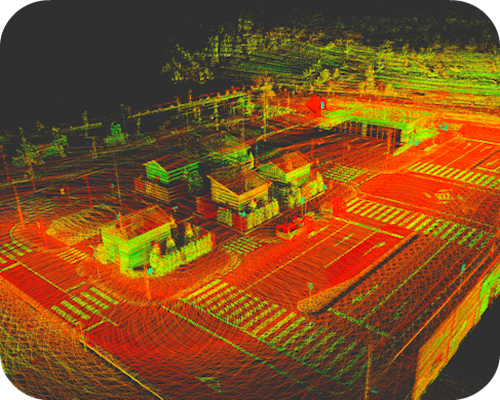
\includegraphics[height=1.6cm,width=.48\linewidth,keepaspectratio]{slam/s05-01.png}\hfill\centering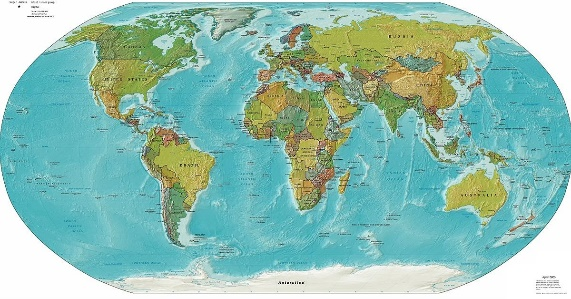
\includegraphics[height=2cm,width=.25\linewidth,keepaspectratio]{slam/s05-03.jpeg}\hfill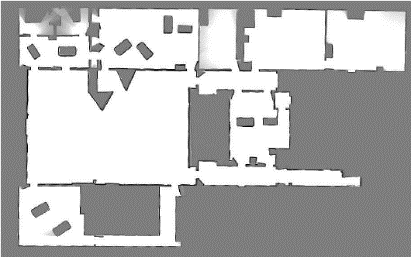
\includegraphics[height=1.6cm,width=.35\linewidth,keepaspectratio]{slam/s05-02.png}\column{.48\textwidth}\centering \begin{block}{Топологические}\begin{itemize}\item Локации и переходы между ними.\item Расстояния могут храниться в связях.\end{itemize}\end{block}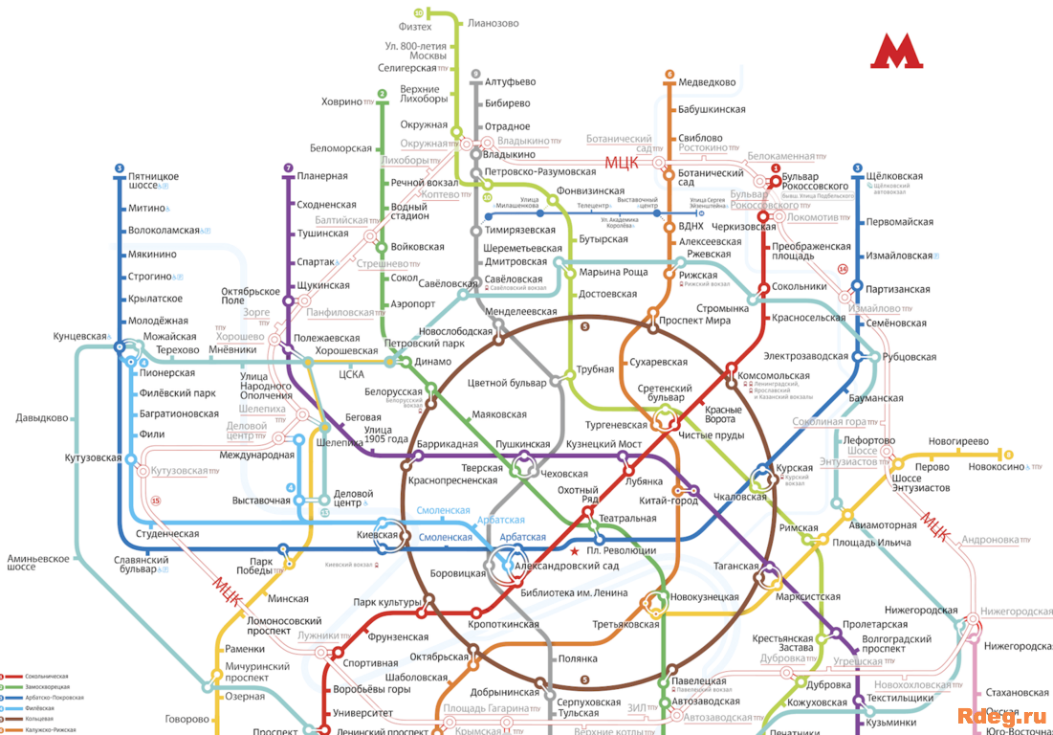
\includegraphics[height=1.7cm,width=.48\linewidth,keepaspectratio]{slam/s05-04.png}\hfill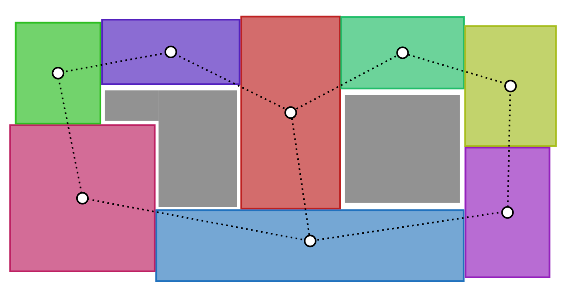
\includegraphics[height=1.7cm,width=.48\linewidth,keepaspectratio]{slam/s05-05.png}\end{columns}
\end{frame}

% Слайд PPTX 6
\begin{frame}
\frametitle{Какие бывают карты?}
\begin{columns}[c]\column{.60\textwidth}\begin{block}{Метрические}\begin{itemize}
\item Карты занятости / проходимости (occupancy grid maps).
\item Карты признаков, особенностей, ориентиров (feature-based, landmark-based maps).
\item Семантические карты: геометрия и смысловые метки объектов.
\end{itemize}
\end{block}\column{.36\textwidth}\centering \begin{block}{Топологические}Графы: узлы — места, рёбра — переходы.\end{block}\end{columns}
\end{frame}

% Слайд PPTX 7
\begin{frame}
\frametitle{Топологические карты}
\begin{columns}[c]\column{.57\textwidth}\small \begin{itemize}
\item Набор локаций (узлов) и переходов между ними (рёбер).
\item Локация — место надёжной локализации или принятия решения о направлении движения, например комната.
\item Переход может содержать закон управления для перемещения между локациями.
\item В больших открытых пространствах такое представление трудно построить.
\end{itemize}
\column{.39\textwidth}\centering \fig[3.8cm]{s07-01.png}\par{\tiny S. Thrun, A. Bücken. Integrating grid-based and topological maps for mobile robot navigation. AAAI, 1996.}\end{columns}
\end{frame}

% Слайд PPTX 8
\begin{frame}
\frametitle{Карты признаков / ориентиров}
\begin{columns}[c]\column{.57\textwidth}\small \begin{itemize}
\item Хранят признаки, заданные координатами в пространстве.
\item Ориентиры: деревья, дорожные знаки, двери, особые точки изображений.
\item Компактное представление пространства.
\end{itemize}
\column{.39\textwidth}\centering \fig[1.8cm]{s08-01.png}\par\medskip\fig[2.3cm]{s08-02.png}\end{columns}
\end{frame}

% Слайд PPTX 9
\begin{frame}
\frametitle{Карты признаков: уточнение оценки}
\begin{columns}[c]\column{.57\textwidth}\small \begin{itemize}
\item Для построения карт признаков используют фильтр Калмана и его модификации.
\item Каждый признак кодируется пространственными координатами.
\item С каждым новым обнаружением оценка положения ориентира уточняется.
\end{itemize}
\column{.39\textwidth}\centering \screenfig[3.8cm]{s09-01.png}{1080bp 220bp 300bp 350bp}\end{columns}
\end{frame}

% Слайд PPTX 10
\begin{frame}
\frametitle{Карты занятости (occupancy grid maps)}
\begin{columns}[c]\column{.57\textwidth}\small \begin{itemize}
\item Один из наиболее распространённых форматов карт.
\item Пространство разбивается на ячейки.
\item Для каждой ячейки оценивается вероятность занятости препятствием.
\item Свободное, занятое и неизвестное пространство различаются.
\end{itemize}
\column{.39\textwidth}\centering \fig[4.1cm]{s10-01.png}\end{columns}
\end{frame}

% Слайд PPTX 11
\begin{frame}
\frametitle{Виды разбиений ячеек}
\centering\screenfig[4.7cm]{s11-01.png}{535bp 245bp 300bp 390bp}
\end{frame}

% Слайд PPTX 12
\begin{frame}
\frametitle{Карты занятости: состояние ячейки}
\begin{columns}[c]\column{.57\textwidth}\small \begin{itemize}
\item Каждая ячейка $m_i\in\{0,1\}$ — бинарная случайная величина.
\item $p(m_i=1)=1$: ячейка занята.
\item $p(m_i=1)=0$: ячейка свободна.
\item $p(m_i=1)=0.5$: нет информации о состоянии ячейки.
\end{itemize}
\column{.39\textwidth}\centering \begin{tikzpicture}[scale=.65]
\fill[gray!50] (0,3) rectangle (1,4);
\fill (1,2) rectangle (3,3);\fill (3,0) rectangle (4,1);
\draw[step=1] (0,0) grid (4,4);
\node[above,font=\scriptsize] at (2,4.2) {Серый: неизвестно};
\node[below,font=\scriptsize,align=center] at (2,-.3) {Чёрный: занято\\Белый: свободно};
\end{tikzpicture}\end{columns}
\end{frame}

% Слайд PPTX 13
\begin{frame}
\frametitle{Карты занятости: независимость ячеек}
\small \begin{itemize}
\item Используем допущение: состояния отдельных ячеек независимы.
\item Тогда вероятность конкретной карты задаётся произведением вероятностей состояний всех её ячеек:
\end{itemize}
\[p(m)=\prod_i p(m_i).\]\begin{center}\begin{tikzpicture}[scale=.5]\fill (0,1) rectangle (1,2);\fill (1,0) rectangle (2,1);\draw (0,0) grid (2,2);\node[right,font=\small] at (3,1) {$p(m)=p(m_1=1)\,p(m_2=0)\,p(m_3=0)\,p(m_4=1)$};\end{tikzpicture}\end{center}
\end{frame}

% Слайд PPTX 14
\begin{frame}
\frametitle{Вероятностная постановка картирования}
\small \begin{itemize}
\item Известны последовательность измерений $z_{1:t}$ и позы робота (сенсора) $x_{1:t}$.
\item Требуется найти наиболее вероятную карту.
\end{itemize}
\[p(m\mid z_{1:t},x_{1:t})\approx\prod_i p(m_i\mid z_{1:t},x_{1:t}).\]\begin{block}{Связанная задача: Structure from Motion (SfM)}Восстановление структуры сцены и движения камеры по последовательности изображений. Совместное уточнение структуры и поз выполняют методом bundle adjustment.\end{block}
\end{frame}

% Слайд PPTX 15
\begin{frame}
\frametitle{Алгоритм hit--miss (counting model)}
\small \begin{itemize}
\item Для каждой ячейки считаем число наблюдений $C_i$.
\item Счётчик $O_i$ увеличиваем на 1, если наблюдаем препятствие, и уменьшаем на 1, если наблюдаем свободное пространство.
\item Вероятность занятости при $C_i>0$:
\end{itemize}
\[p(m_i=1)=\frac{O_i+C_i}{2C_i}.\]\begin{itemize}
\item Эквивалентно: доля попаданий среди всех наблюдений ячейки.
\item Если $C_i=0$, сохраняем априорную вероятность (обычно $0.5$).
\end{itemize}
\end{frame}

% Слайд PPTX 16
\begin{frame}
\frametitle{Картирование с обратной моделью сенсора}
\small \begin{columns}[c]\column{.62\textwidth}Обратная модель: $p(m_i=1\mid z_t,x_t)$.
\[l_{t,i}=\log\frac{p(m_i=1\mid z_{1:t},x_{1:t})}{1-p(m_i=1\mid z_{1:t},x_{1:t})}.\]
Для ячеек в поле зрения:
\[l_{t,i}=l_{t-1,i}+\operatorname{logit}p(m_i=1\mid z_t,x_t)-l_0.\]
Для остальных: $l_{t,i}=l_{t-1,i}$.
\par\medskip В логарифмических шансах обновление — сложение.\column{.34\textwidth}\centering \fig[2.8cm]{s16-02.png}\par\scriptsize Пример простой модели измерения сонара.\par\medskip Свободная область перед отражением; занятая область около измеренной дальности.\end{columns}\source{О. Шипитько, МФТИ, 2020; иллюстрация: Gian Diego Tipaldi, Wolfram Burgard.}
\end{frame}

% Слайд PPTX 17
\begin{frame}
\frametitle{Ограничения обратной модели сенсора}
\small \begin{itemize}
\item Независимое обновление ячеек не учитывает зависимости между ними.
\item Противоречащие измерения могут приводить к несогласованной карте.
\end{itemize}
\begin{center}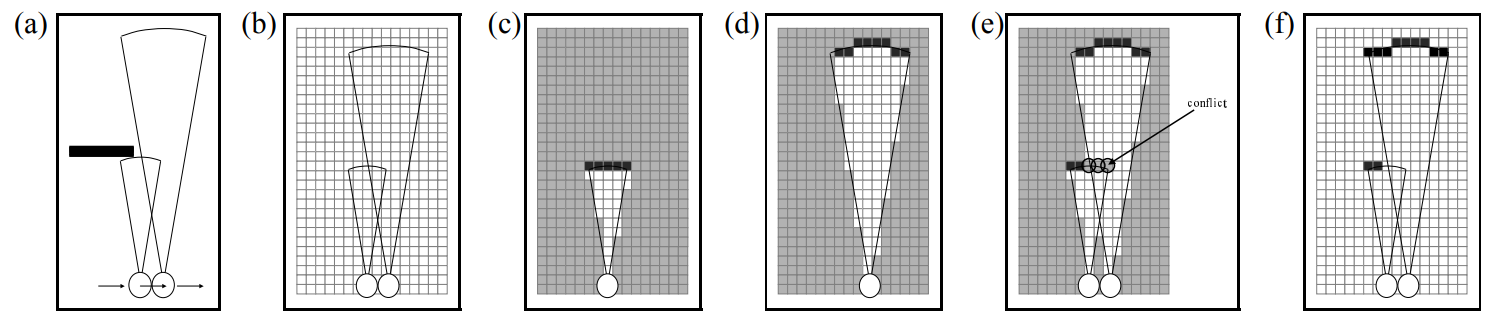
\includegraphics[height=1.35cm,width=.9\linewidth,keepaspectratio]{slam/s17-01.png}\end{center}\begin{itemize}
\item Альтернатива: оптимизация всей карты с прямой моделью сенсора.
\end{itemize}
\[m^*=\arg\max_m p(z_{1:t}\mid m,x_{1:t}).\]
\end{frame}

% Слайд PPTX 18
\begin{frame}
\frametitle{Объединение нескольких измерений}
\begin{columns}[c]\column{.48\textwidth}\small Каждая ячейка обновляется после измерения бинарным фильтром Байеса (Moravec, 1985).\[M_i^{(t)}=\frac{p_i^{(t)}}{1-p_i^{(t)}},\qquad p_i^{(t)}=\frac{M_i^{(t)}}{1+M_i^{(t)}}.\]\[M_i^{(t+1)}=M_i^{(t)}\frac{P_i}{1-P_i}\quad(p_0=0.5).\]$P_i$ — вероятность занятости по новому измерению; $M_i$ — шансы занятости.\column{.48\textwidth}\centering \fig[3.6cm]{s18-01.png}\end{columns}\source{Источник: University of Washington, CSE571, 2015. \href{https://courses.cs.washington.edu/courses/cse571/15au/slides/09-occupancy-mapping.pdf}{Occupancy Mapping}.}
\end{frame}

% Слайд PPTX 19
\begin{frame}
\frametitle{Форматы пространственных карт}
\fontsize{8}{9.5}\selectfont
\begin{columns}[T]
\column{.31\textwidth}
\begin{block}{Облако точек}
Без дискретизации; область карты заранее не ограничена.\par\medskip
Память растёт с данными. Свободное и неизвестное пространство явно не представлены.
\end{block}
\centering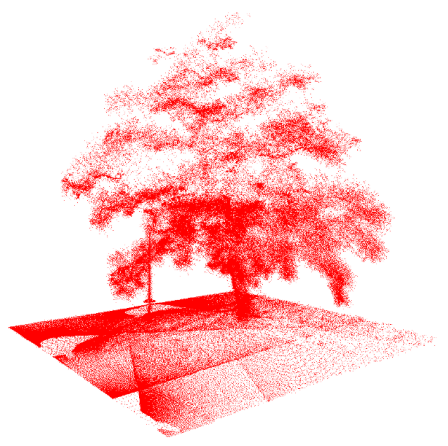
\includegraphics[height=1.35cm]{slam/s19-02.png}
\column{.31\textwidth}
\begin{block}{2.5D: карта высот}
2D-сетка; в ячейке — высота (или несколько высот) и уверенность.\par\medskip
Экономна по памяти. Ограниченно описывает 3D; свободное и неизвестное пространство не различаются явно.
\end{block}
\centering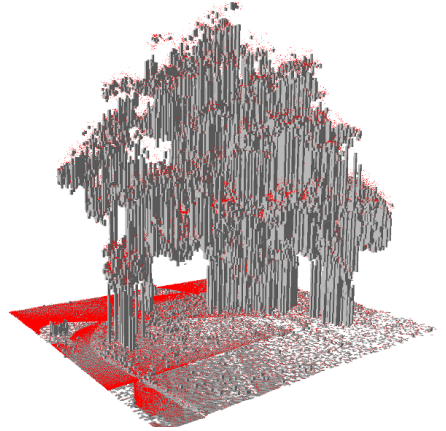
\includegraphics[height=1.35cm]{slam/s19-03.png}
\column{.34\textwidth}
\begin{block}{Воксели и октодеревья}
Полная вероятностная 3D-модель. Рекурсивное деление объёма на 8 частей; память выделяется по мере необходимости.\par\medskip
Несколько разрешений; экономия памяти. Сложнее реализация и обновление.
\end{block}
\centering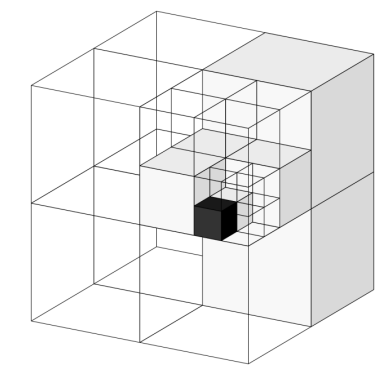
\includegraphics[height=1.1cm]{slam/s19-04.png}\hfill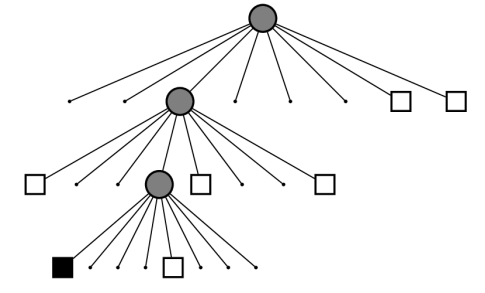
\includegraphics[height=1.1cm]{slam/s19-05.png}
\end{columns}
\vspace{1mm}\centering
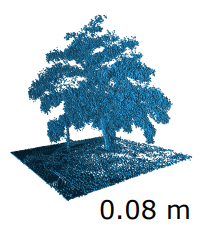
\includegraphics[height=.9cm]{slam/s19-01.png}\quad
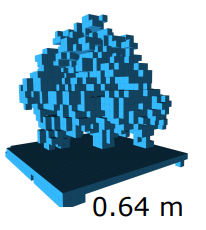
\includegraphics[height=.9cm]{slam/s19-06.png}\quad
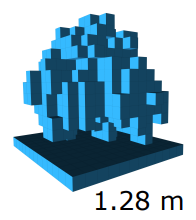
\includegraphics[height=.9cm]{slam/s19-07.png}
\source{\href{https://github.com/OctoMap/octomap}{OctoMap}; University of Washington, CSE571, Occupancy Mapping, 2015.}
\end{frame}

% Слайд PPTX 26
\begin{frame}
\frametitle{SLAM: совместная оценка траектории и карты}
\small \begin{itemize}
\item Локализация и картирование — задачи оценки состояния по данным сенсоров.
\item В локализации состояние — поза или траектория; в картировании — карта.
\item Одни и те же сенсорные данные позволяют оценивать их совместно.
\end{itemize}
\begin{block}{Simultaneous Localization And Mapping}
Совместно оцениваем траекторию $x_{0:t}$ и карту $m$:
\[p(x_{0:t},m\mid z_{1:t},u_{0:t-1}).\]
Наблюдения: $z_k=h_k(x_i,m_j)+v_k$.
\end{block}
SfM — связанная задача восстановления структуры сцены и движения камеры; bundle adjustment уточняет позы и 3D-точки.
\source{К. В. Миронов, 2023; Gonzalo Ferrer, «SLAM: Problem Elements».}
\end{frame}

% Слайд PPTX 27
\begin{frame}
\frametitle{SLAM как задача оптимизации}
\fontsize{9}{10.5}\selectfont \begin{columns}[c]\column{.49\textwidth}Обозначим все позы и ориентиры через $\mathcal X$, наблюдения — через $\mathcal Z$.
\[
\begin{aligned}
\mathcal X^*&=\arg\max_{\mathcal X}p(\mathcal X\mid\mathcal Z)\\
&=\arg\min_{\mathcal X}\{-\log p(\mathcal X,\mathcal Z)\}.
\end{aligned}
\]
При независимых гауссовских ошибках:
\[\mathcal X^*=\arg\min_{\mathcal X}\sum_k\|h_k(\mathcal X)-z_k\|_{\Sigma_k}^2,\]
где $\|e\|_{\Sigma}^2=e^\top\Sigma^{-1}e$. Априорные ограничения включаем в сумму.\column{.47\textwidth}\centering Линеаризация и объединение невязок:
\[\min_{\Delta x}\|W^{1/2}(A\Delta x-b)\|_2^2.\]
Нормальные уравнения:
\[\underbrace{A^\top W A}_{\text{информационная матрица}}\Delta x=A^\top Wb.\]
\begin{itemize}
\item Решаем систему и обновляем оценку.
\item Повторяем линеаризацию (Гаусс--Ньютон / Левенберг--Марквардт).
\item Фиксируем систему координат: например, первую позу.
\end{itemize}\end{columns}\source{По материалам Gonzalo Ferrer, «SLAM: Solving the problem» (в исходнике — скриншоты вывода).}
\end{frame}

% Слайд PPTX 28
\begin{frame}
\frametitle{Визуальные методы SLAM}
\fontsize{8}{9.4}\selectfont
\begin{columns}[T]
\column{.48\textwidth}
\begin{block}{Разреженные + косвенные (sparse + indirect)}
Сопоставляют ключевые точки; минимизируют геометрическую ошибку, например ошибку репроекции. Геометрия оценивается по соответствиям.
\end{block}
\href{https://arxiv.org/pdf/1610.06475.pdf}{ORB-SLAM2} (Universidad de Zaragoza): моно-, стерео-, RGB-D.\par
\href{https://arxiv.org/pdf/1910.01122.pdf}{OpenVSLAM} (Tokyo Institute of Technology).\par
\href{https://introlab.3it.usherbrooke.ca/mediawiki-introlab/images/7/7a/Labbe18JFR_preprint.pdf}{RTAB-Map} (Université de Sherbrooke): одометрия и картирование по камере и/или лидару.
\begin{block}{Плотные + косвенные (dense + indirect)}
Геометрия восстанавливается вместе с плотным оптическим потоком. Ошибка соответствий сочетается с ограничениями гладкости потока.
\end{block}
\column{.48\textwidth}
\begin{block}{Разреженные + прямые (sparse + direct)}
Минимизируют фотометрическую ошибку непосредственно по интенсивностям выбранных пикселей; без плотной регуляризации геометрии.
\end{block}
\href{https://vision.in.tum.de/media/spezial/bib/engel2016dso.pdf}{DSO} (Technical University of Munich); \href{https://vision.in.tum.de/_media/research/vslam/stereo-dso/wang2017stereodso.pdf}{Stereo DSO}.\par
\href{https://arxiv.org/abs/1807.02570}{DVSO}: Deep Virtual Stereo Odometry.\par
\href{https://arxiv.org/abs/2003.01060}{D3VO}: Deep Depth, Deep Pose and Deep Uncertainty for Monocular Visual Odometry.
\begin{block}{Плотные + прямые (dense + direct)}
Фотометрическая ошибка и априорные ограничения геометрии позволяют оценивать плотную или полуплотную структуру сцены.
\end{block}
\end{columns}
\source{Классификация и примеры из исходной лекции (2023). DSO и его варианты — методы визуальной одометрии.}
\end{frame}

\begin{frame}
	\frametitle{SLAM в ROS2}
	\begin{block}{Типы сообщений}
		\begin{itemize}
			\item \cmd{sensor\_msgs/PointCloud2} - облако точек (может передавться как облако точек с одного лидара, так и 3D карта);
			\item \cmd{nav\_msgs/OccupancyGrid} - карта занятости.
		\end{itemize}
	\end{block}
	
	\begin{block}{Пакет \cmd{slam\_toolbox}}
		Основан на алгоритме GMapping. Построение карты с нуля, сохранение карты, загрузка сохраненной карты, публикация карты в виде OccupancyGrid.
	\end{block}
\end{frame}

\begin{frame}
	\frametitle{Полезные материалы}
	\small
	\begin{itemize}
		
		\item  
		\href{https://github.com/literator1996/veroyatnostnaya_robototehnica/tree/master}{С. Трун, В. Бургард, Д. Фокс. Вероятностная робототехника (перевод на русский язык)}.
		\item\href{https://github.com/oleg-Shipitko/mipt\_wheeled\_robots\_modeling\_2022/blob/main/slides/Lecture\%205.\%20Mapping.pdf}{Лекции О. Шипитко (МФТИ). Лекция 5. Картирование}.  
	\end{itemize}
\end{frame}

\begin{frame}
	\begin{center}
		\Large Спасибо за внимание!
	\end{center}
	\vfill
\end{frame}

\end{document}
